\documentclass[12pt,spanish]{article}
\usepackage[utf8]{inputenc}
\usepackage{babel}
\usepackage{listings}
\usepackage{mathpazo}
\usepackage{enumitem}
\usepackage{courier}
\usepackage{textcomp}
\usepackage{xcolor}
\usepackage{parskip}
\usepackage{fullpage}
\usepackage{tikz}

\newcommand{\onelinerule}{\rule[2.3ex]{0pt}{0pt}}
\newcommand{\twolinerule}{\rule[6.2ex]{0pt}{0pt}}
\newcommand{\respuesta}{\framebox[\textwidth]{\twolinerule}}
\newcommand{\nombre}{%
  \begin{tikzpicture}[xscale=.4,yscale=.7]
    \draw (0, 0) rectangle (22, 1);
  \end{tikzpicture}%
}
%\newcommand{\rol}   {\framebox[0.3\textwidth]{\onelinerule}}
\newcommand{\rol}{%
  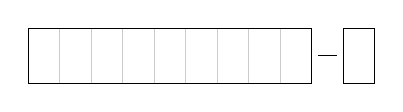
\begin{tikzpicture}[xscale=.4,yscale=.7]
    \draw[gray!40] ( 0, 0) grid      ( 9, 1);
    \draw          ( 0, 0) rectangle ( 9, 1);
    \draw          (10, 0) rectangle (11, 1);
    \draw (9 + .2, .5) -- (10 - .2, .5);
  \end{tikzpicture}%
}
\newcommand{\li}{\lstinline}
\providecommand{\pond}[1]{[{\small\textbf{#1\%}}]}

\lstdefinelanguage{py}{%
  classoffset=0,%
    morekeywords={%
      False,class,finally,is,return,None,continue,for,lambda,try,%
      True,def,from,nonlocal,while,and,del,global,not,with,print,%
      as,elif,if,or,yield,assert,else,import,pass,break,except,in,raise},%
    keywordstyle=\color{black!80}\bfseries,%
  classoffset=1,
    morekeywords={int,float,str,abs,len,raw_input,exit,range,min,max,%
      set,dict,tuple,list,bool,complex,round,sum,all,any,zip,map,filter,%
      sorted,reversed,dir,file,frozenset,open,%
      array,zeros,ones,arange,linspace,eye,diag,dot},
    keywordstyle=\color{black!50}\bfseries,%
  classoffset=0,%
  sensitive=true,%
  morecomment=[l]\#,%
  morestring=[b]',%
  morestring=[b]",%
  stringstyle=\em,%
}

\lstdefinelanguage{testcase}{%
  moredelim=[is][\bfseries]{`}{`},%
  backgroundcolor=\color{gray!20},%
}

\lstdefinelanguage{file}{%
  frame=single,%
}

\lstset{language=py}
\lstset{basicstyle=\ttfamily}
\lstset{columns=fixed}
\lstset{upquote=true}
\lstset{showstringspaces=false}
\lstset{rangeprefix=\#\ }
\lstset{includerangemarker=false}

\newlist{certamen}{enumerate}{1}
\setlist[certamen]{%
  label=\arabic*.,
  font=\LARGE\bfseries,%
  labelindent=-.5in,%
  leftmargin=0pt,%
  labelsep=1em%
}



\lstset{language=file,frame=single}

\begin{document}
  \thispagestyle{empty}
  \section*{Lunes 26 de noviembre}

  El \emph{Combate Naval} es un juego de papel y lápiz
  en que cada jugador pone una flota de barcos
  en una grilla de \(10\times 10\).

  La flota consiste de
  un portaaviones de tamaño 5,
  dos acorazados de tamaño 4,
  tres submarinos de tamaño 3
  y cuatro cruceros de tamaño 2.
  Los barcos pueden ponerse horizontal o verticalmente,
  y no pueden tocarse entre ellos ni siquiera en diagonal.

  A continuación vemos un ejemplo de tablero que podría llenar un jugador,
  y a su derecha cuál es el formato de archivo
  que usaremos para representarlo:

  \tikzstyle{ship}=[draw=black, fill=gray]
  \begin{minipage}[T]{0.45\textwidth}
    \begin{tikzpicture}[scale=.5,yscale=-1]
      \foreach\i in {0,...,9} \node[font=\small] at (-0.5, \i + 0.5) {\i};
      \foreach\j in {0,...,9} \node[font=\small] at (\j + 0.5, -0.5) {\j};
      \draw (0, 0) grid (10, 10);
      \filldraw[ship] (2, 2) rectangle ++(1, 5);
      \filldraw[ship] (8, 3) rectangle ++(1, 4);
      \filldraw[ship] (4, 1) rectangle ++(4, 1);
      \filldraw[ship] (0, 2) rectangle ++(1, 3);
      \filldraw[ship] (0, 0) rectangle ++(3, 1);
      \filldraw[ship] (4, 4) rectangle ++(3, 1);
      \filldraw[ship] (9, 0) rectangle ++(1, 2);
      \filldraw[ship] (0, 9) rectangle ++(2, 1);
      \filldraw[ship] (5, 8) rectangle ++(2, 1);
      \filldraw[ship] (8, 8) rectangle ++(1, 2);
    \end{tikzpicture}
  \end{minipage}
  \begin{minipage}[T]{0.45\textwidth}
    \vspace{3ex}
    \lstinputlisting[language=file]{a.txt}
  \end{minipage}

  Cada línea del archivo representa un barco de la flota,
  y contiene los siguientes datos:
  tipo de barco,
  fila de la primera celda,
  columna de su primera celda
  y dirección del barco (\verb+V+ si es vertical y \verb+H+ si es horizontal).

  \begin{enumerate}[leftmargin=0pt]

    \item
      \begin{minipage}[t]{0.6\textwidth}
        \parskip=2ex

        Escriba un programa llamado \verb+crear_tablero.py+
        que le pregunte al usuario
        el nombre del archivo que contiene la flota,
        y cree un nuevo archivo con un mapa del tablero
        como el de la derecha.

        El nombre del nuevo archivo debe ser el del archivo de barcos
        precedido de «\verb+tablero-+».
        (Por ejemplo, \verb+a.txt+ \(\to\) \verb+tablero-a.txt+).

        Al ejecutar el programa debe verse lo siguiente:

        \lstinputlisting[language=testcase]{caso.txt}
      \end{minipage}
      \hfill
      \begin{minipage}[t]{0.35\textwidth}
        \lstinputlisting[language=file]{tablero-a.txt}
      \end{minipage}

      Le recomiendo que antes de crear el nuevo archivo
      llene un conjunto con las coordenadas de todas las casillas del tablero
      que están ocupadas.

    \item
      Escriba un programa llamado \verb+validar.py+
      que le pregunte al usuario el nombre de un archivo de barcos
      y le diga los errores que tiene la flota.
      Por ejemplo:
      \lstinputlisting[language=testcase]{caso-validar.txt}

  \end{enumerate}


\end{document}

